\lstinputlisting[language=bash,basicstyle=\small]{python_codes/fieldstone_40/keywords}

\begin{center}
Code at \url{https://github.com/cedrict/fieldstone/tree/master/python_codes/fieldstone_40}
\end{center}

\par\noindent\rule{\textwidth}{0.4pt}
%%%%%%%%%%%%%%%%%%%%%%%%%%%%%%%%%%%%%%%%%%%%%%%%%%%%%%%%%%%%%%%%%%%%%%%%%%%%%%%%%%%%%%%%%%%%

This benchmark is carried out in \textcite{deka08} (2008), \textcite{gery10} (2010) and \textcite{thie11} (2011) 
and is based on the analytical solution by \textcite{ramb68} (1968). 
It consists of a buoyancy-driven two-layer system driven. 
The domain is a square of size $512\times512$km. 
Free slip are imposed on the sides while no-slip boundary conditions are imposed on the
top and the bottom of the box.

Fluid 1 $(\rho_1,\eta_1)$ of thickness $h_1$ overlays 
fluid 2 $(\rho_2,\eta_2)$ of thickness $h_2$ (with $h_1+h_2=L_y$).
An initial sinusoidal disturbance of the interface between these
layers is introduced and is characterised by an amplitude $\Delta$ and a
wavelength $\lambda=L_x/2$ as shown here: 

\begin{center}
a) 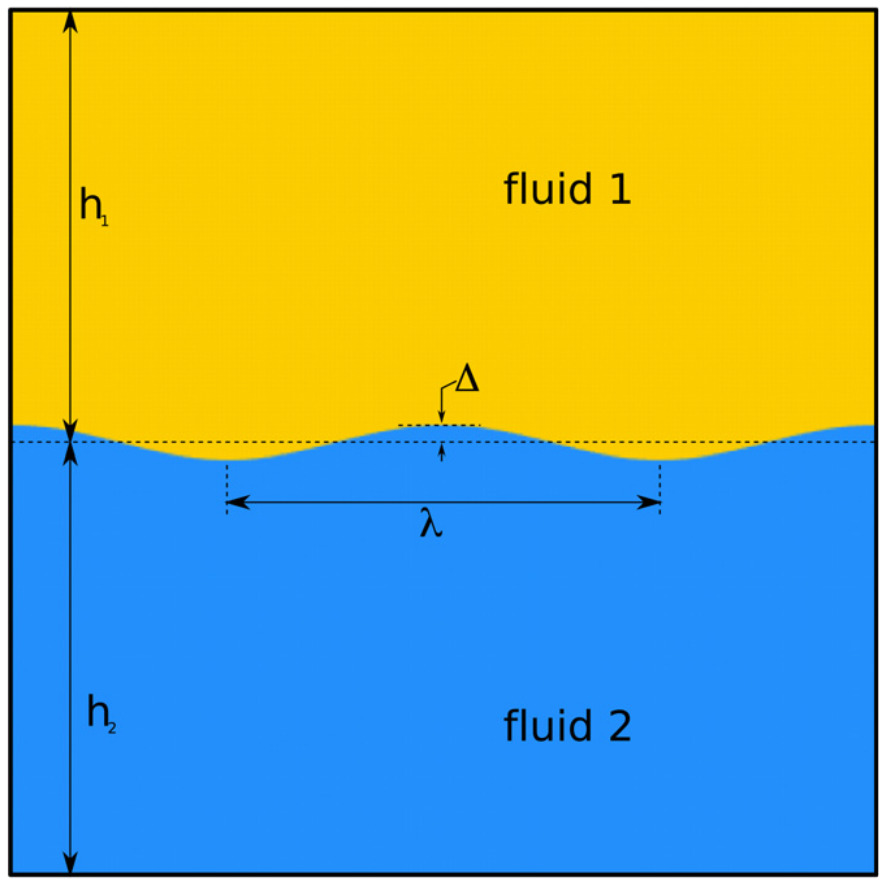
\includegraphics[width=0.38\textwidth]{python_codes/fieldstone_40/images/setup}
b) 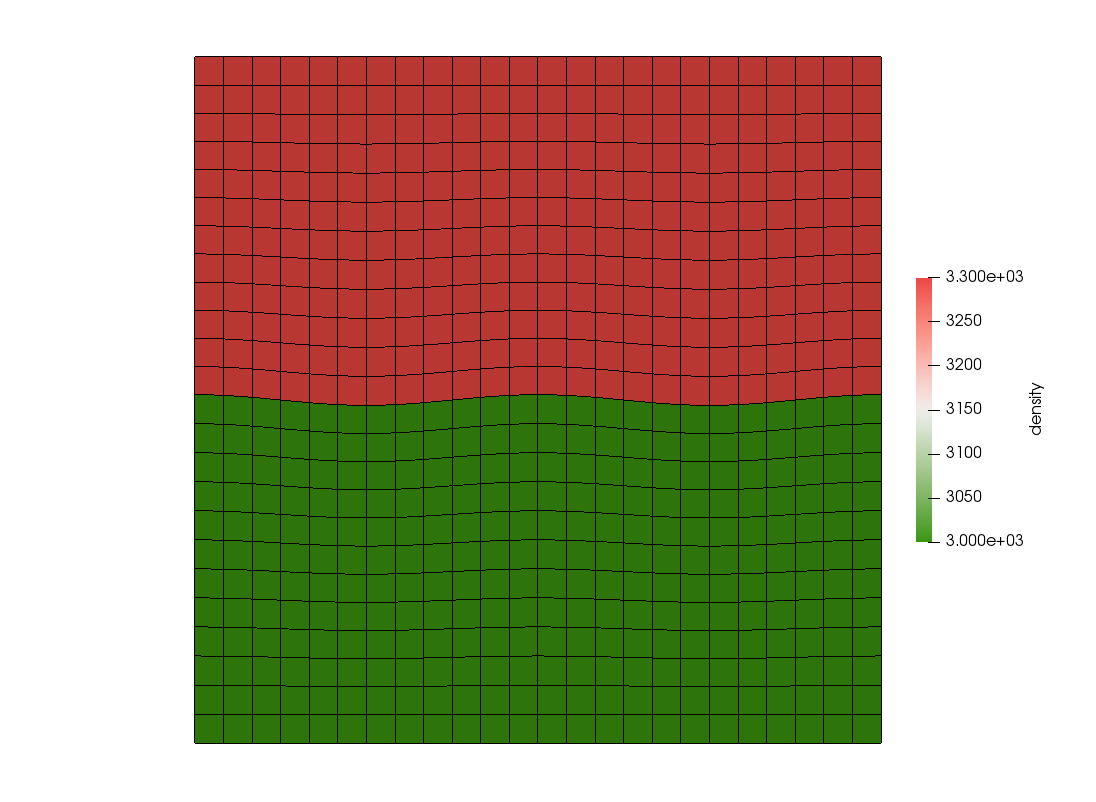
\includegraphics[width=0.55\textwidth]{python_codes/fieldstone_40/images/dens}\\
{\captionfont  a) Setup of the experiment, taken from \cite{thie11}; b) grid setup for 24$\times$24 grid.} 
\end{center}

Under this condition, the velocity of the diapiric growth
$v_y$ is given by the relation
\[
\frac{v_y}{\Delta} = - K \frac{\rho_1-\rho_2}{2 \eta_2} h_2 g
\]
with the dimensionless growth factor $K$ being
\[
K=\frac{-d_{12}}{c_{11}j_{22}-d_{12}i_{21}}
\]
and 
\begin{eqnarray}
c_{11} &=& \frac{\eta_1 2 \phi_1^2}{\eta_2(\cosh 2\phi_1 - 1 - 2\phi_1^2)} - \frac{2\phi_2^2}{\cosh 2\phi_2 - 1 - 2 \phi_2^2}\\
d_{12} &=& \frac{\eta_1(\sinh 2\phi_1 -2\phi_1)}{\eta_2(\cosh 2\phi_1 -1 -2\phi_1^2)} + \frac{\sinh 2\phi_2 - 2\phi_2}{\cosh 2\phi_2 -1 -2\phi_2^2} \\
i_{21} &=& \frac{\eta_1\phi_2 (\sinh 2 \phi_1 + 2 \phi_1)}{\eta_2(\cosh 2\phi_1 -1 -2\phi_1^2)} 
+ \frac{\phi_2 (\sinh 2\phi_2 + 2\phi_2)}{\cosh 2\phi_2 -1 -2\phi_2^2} \\
j_{22} &=& \frac{\eta_1 2 \phi_1^2 \phi_2}{\eta_2(\cosh 2\phi_1 -1-2\phi_1^2)} - \frac{2\phi_2^3}{ \cosh 2\phi_2 -1 -2\phi_2^2}\\
\phi_1&=&\frac{2\pi h_1}{\lambda}\\
\phi_2&=&\frac{2\pi h_2}{\lambda}
\end{eqnarray}


\begin{center}
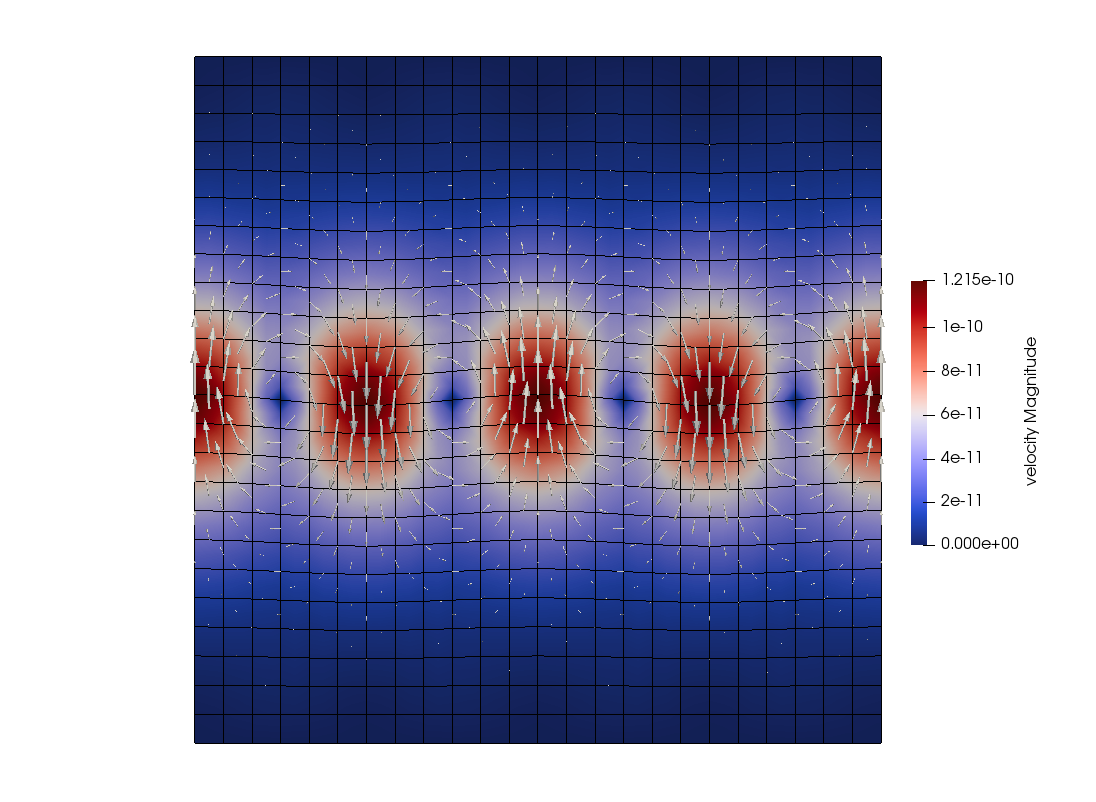
\includegraphics[width=7cm]{python_codes/fieldstone_40/images/vel}
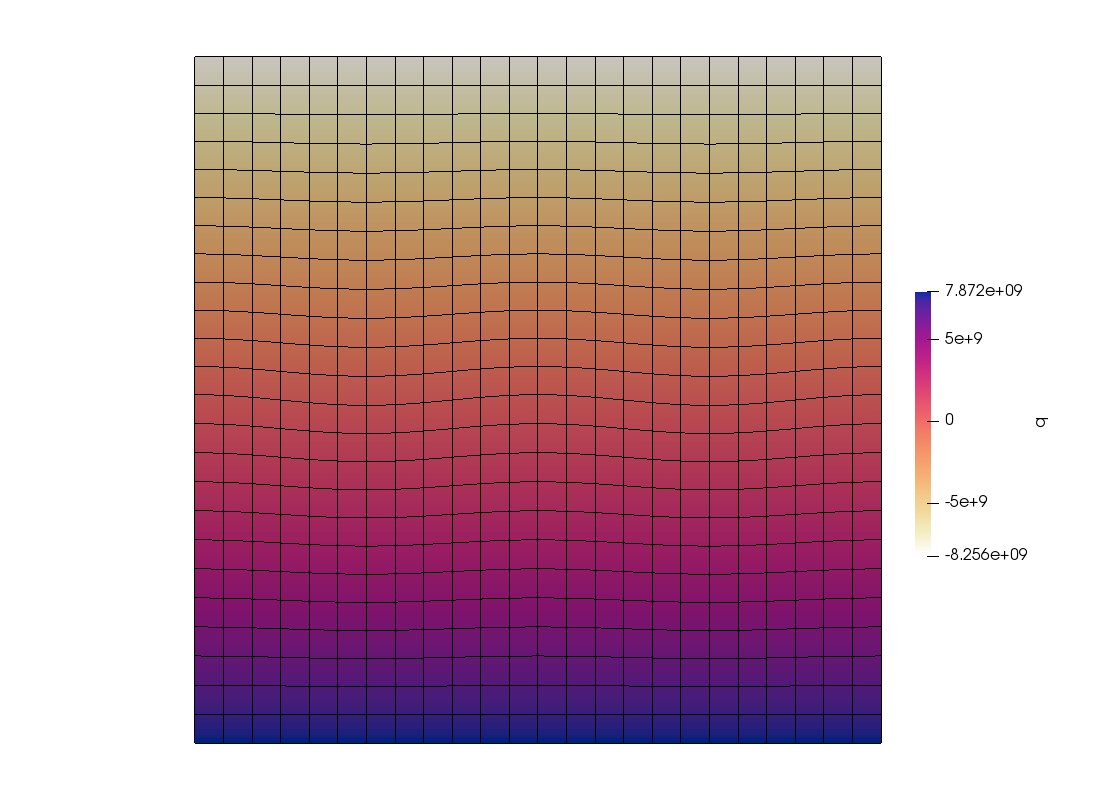
\includegraphics[width=7cm]{python_codes/fieldstone_40/images/p}
\end{center}


\begin{center}
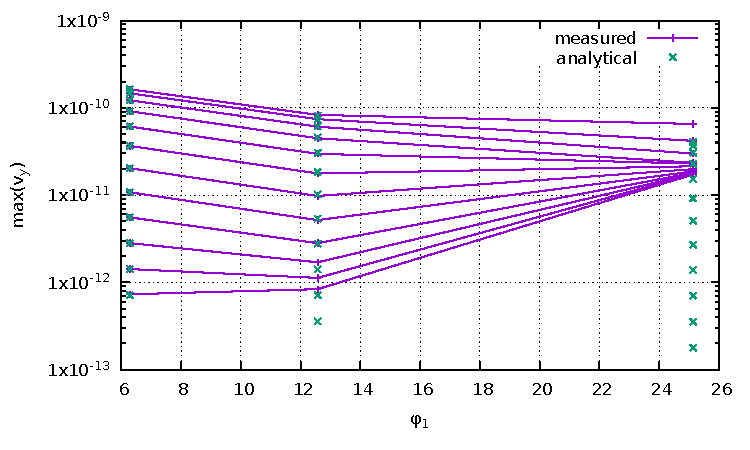
\includegraphics[width=5cm]{python_codes/fieldstone_40/images/plot24x24}
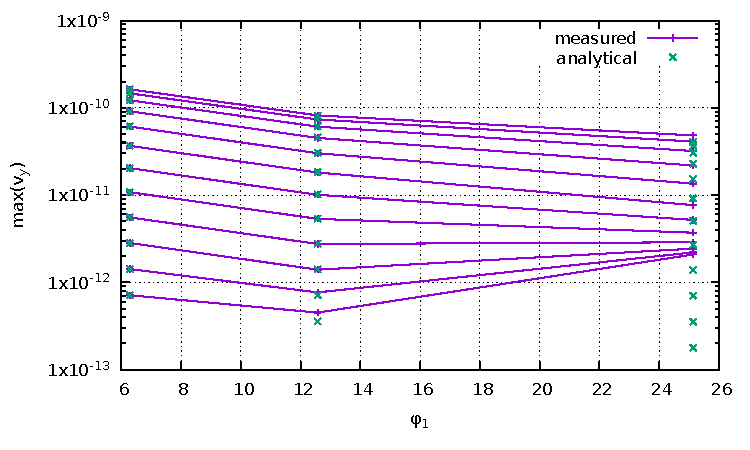
\includegraphics[width=5cm]{python_codes/fieldstone_40/images/plot32x32}
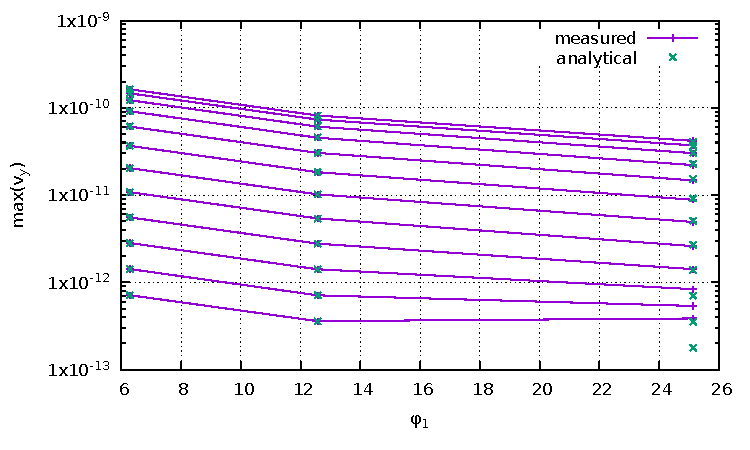
\includegraphics[width=5cm]{python_codes/fieldstone_40/images/plot48x48}\\
{\captionfont  Left: 24$\times$24 elements, middle: 32$\times$32; right: 48$\times$48. We see that 
increasing resolution yields more accurate results in the cases of short wavelength 
perturbations (points on the right on the plots).\\  
Note that in \cite{thie11} I fixed $\lambda=L_x/2$ and varied $L_x$. Here I keep $L_x$ fixed
and vary $\lambda=L_x/2,L_x,4,L_x/8$. Each line corresponds to a different value of the viscosity $\eta_2$.} 
\end{center}


